\section{Experiments}
\label{sec:experiments}

\subsection{Challenges and Learning Experiences}

\subsubsection{Writing My First Extensive ESP-IDF Project}
This project was my first experience writing such an extensive program using the ESP-IDF framework, and it was both challenging and rewarding. I had never worked with the ESP32 in such depth before, and the complexity of integrating various hardware components and managing their interactions made this project a great learning experience. Compared to using the Arduino framework where many things are abstracted and you can use libraries for most tasks.

\subsubsection{Working with Interrupts}
One of the most significant challenges I faced was working with interrupts. Interrupts were a fairly new concept to me in practice, and I had to ensure that each component was correctly handled through interrupt service routines (ISRs). These are critical for real-time response, especially for buttons and sensors, but understanding how to manage them effectively required careful study and implementation. Despite the steep learning curve, I now feel more comfortable with this aspect of embedded systems development.

\subsubsection{OLED Display Challenges}
The OLED display was another area where I encountered difficulties. I attempted to control the display without relying on an external library, which I thought would give me more flexibility. However, I struggled to get the display to function properly, as handling the low-level communication with the I2C interface and sending commands manually proved more complicated than expected. I wish I could've gotten this to work.

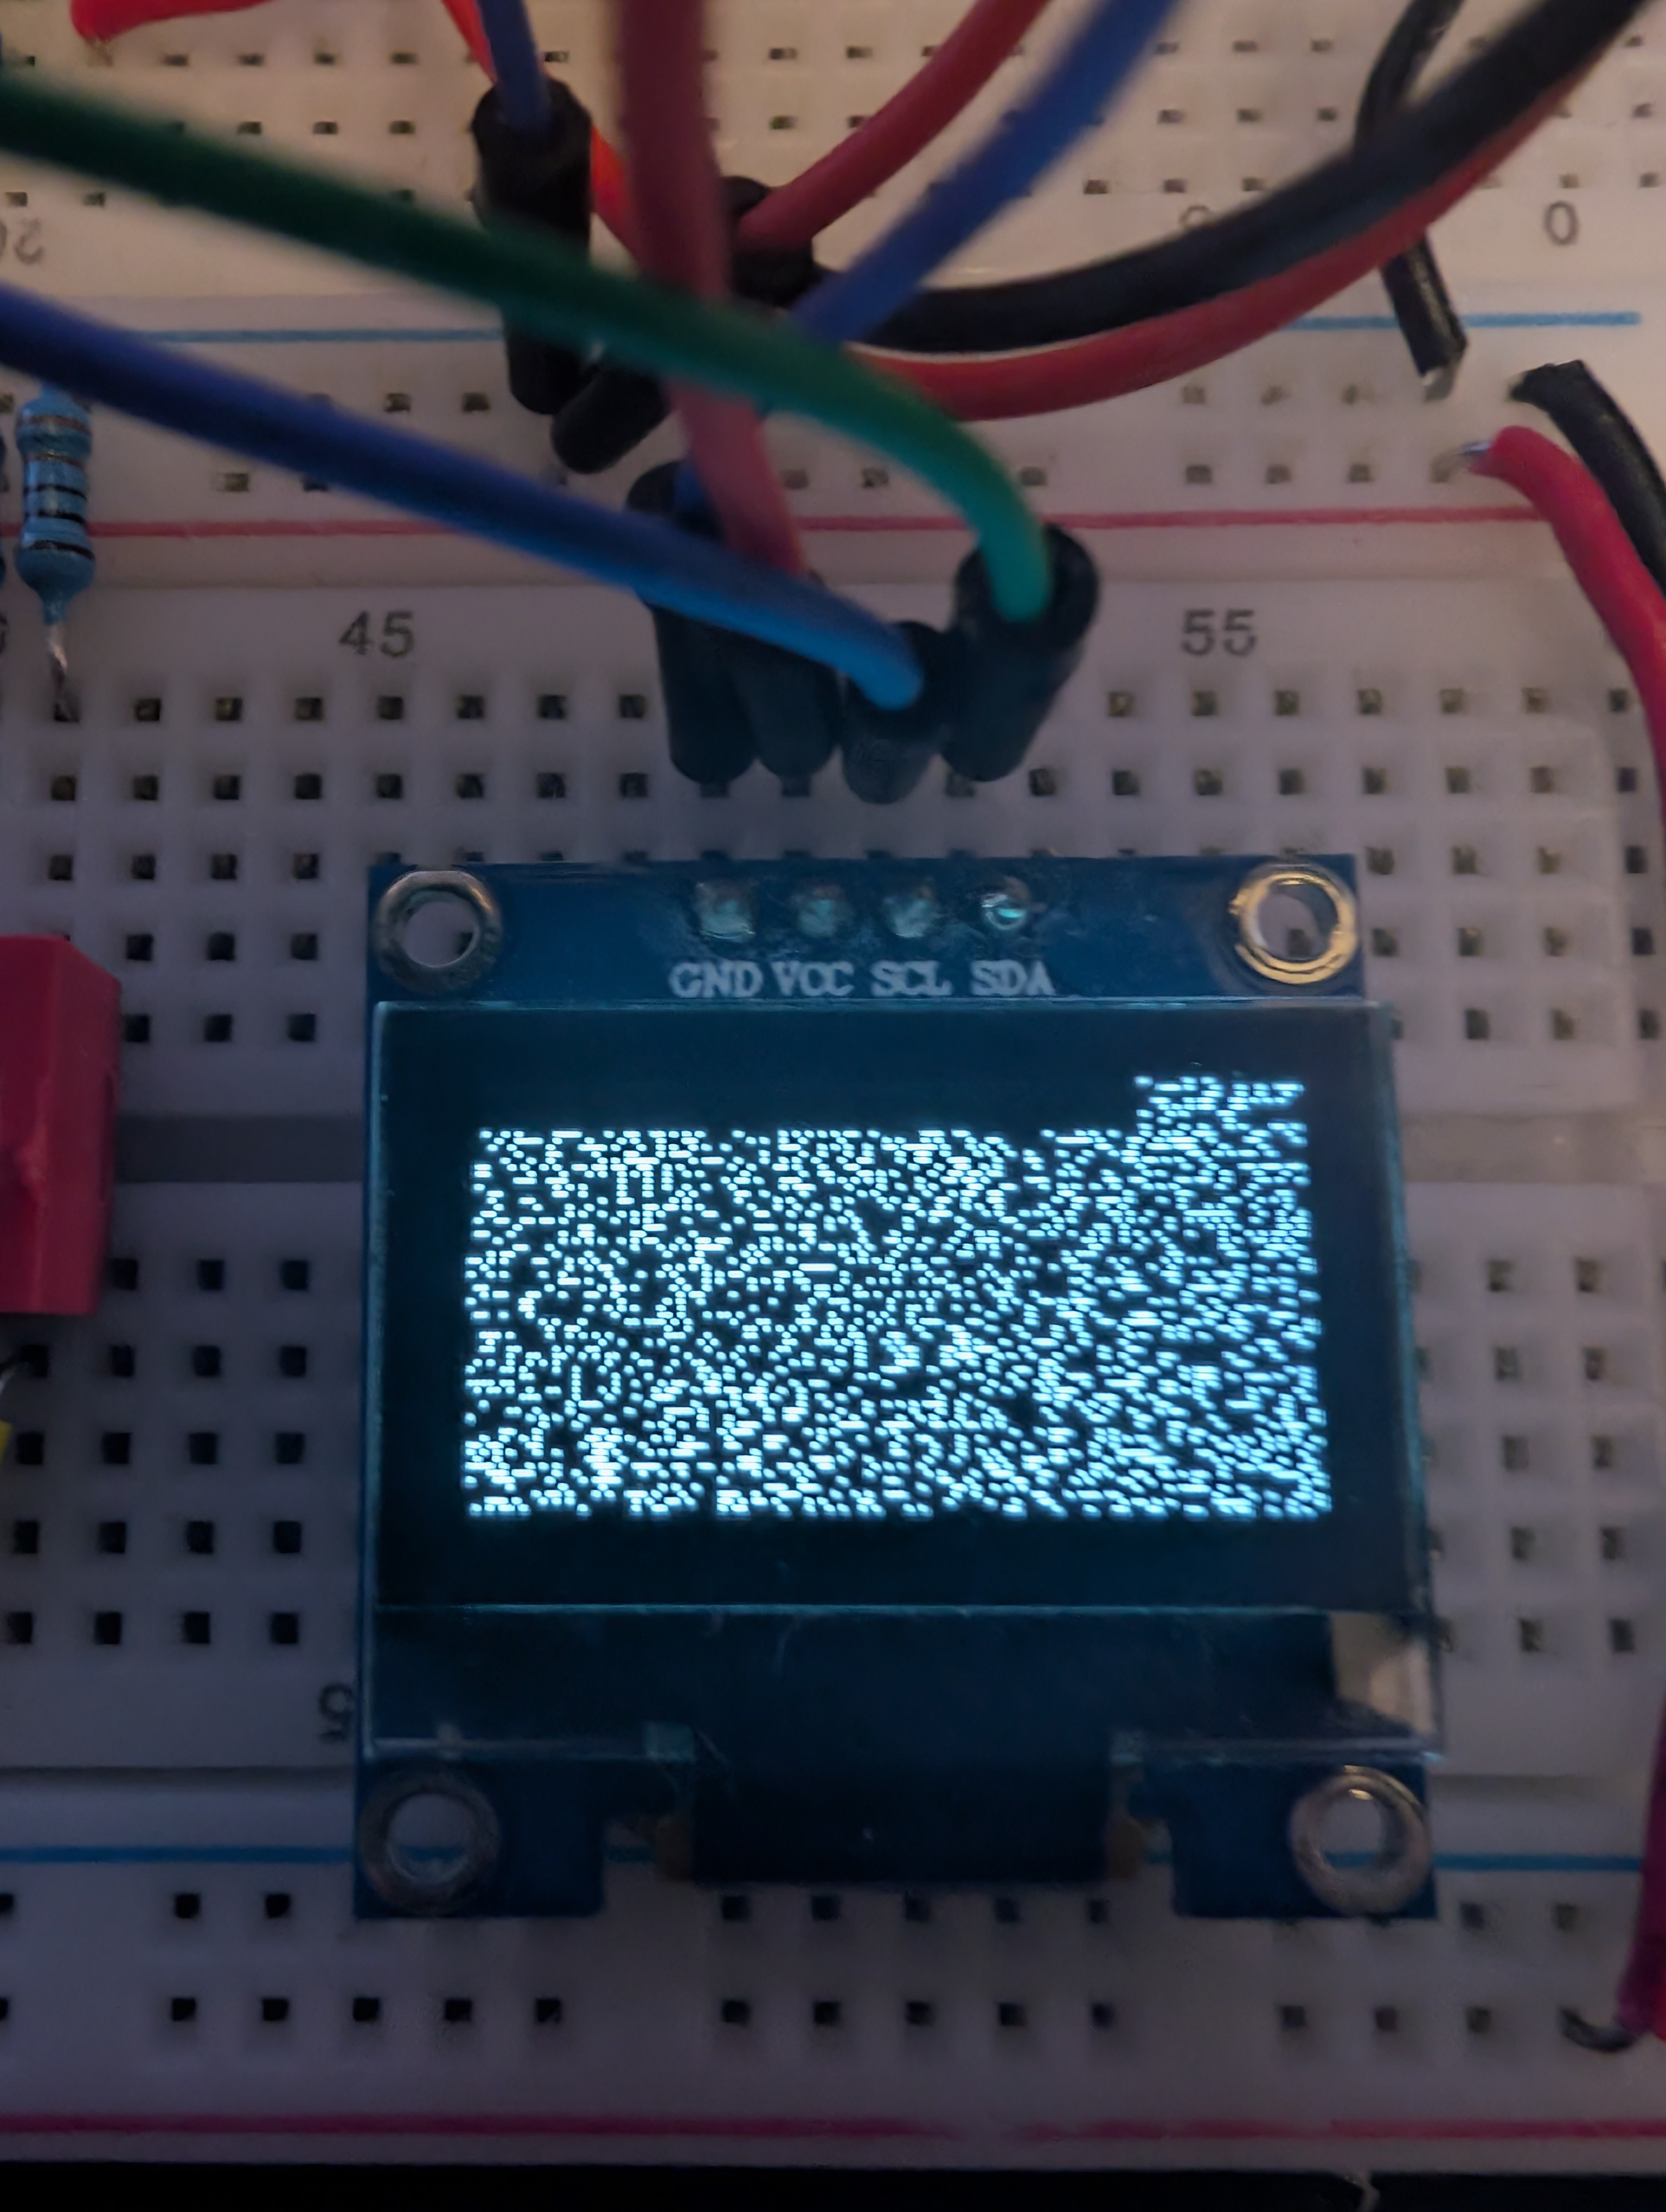
\includegraphics[scale=0.05]{img/oled.jpg}

\subsubsection{Multithreading with FreeRTOS Tasks}
Multithreading using tasks in FreeRTOS was another unfamiliar area for me. Managing multiple tasks concurrently, such as reading sensor values, controlling the motor, and handling button presses. Learning this concept was really helpful.

\subsubsection{Component Configuration}
Another significant part of the project involved configuring all the components from scratch. I was able to get deeply involved in the technical details of each hardware component, from setting up the GPIOs for switches and LEDs to configuring the motor driver and sensor interfaces. I learned the importance of proper component initialization and configuration for reliable operation.

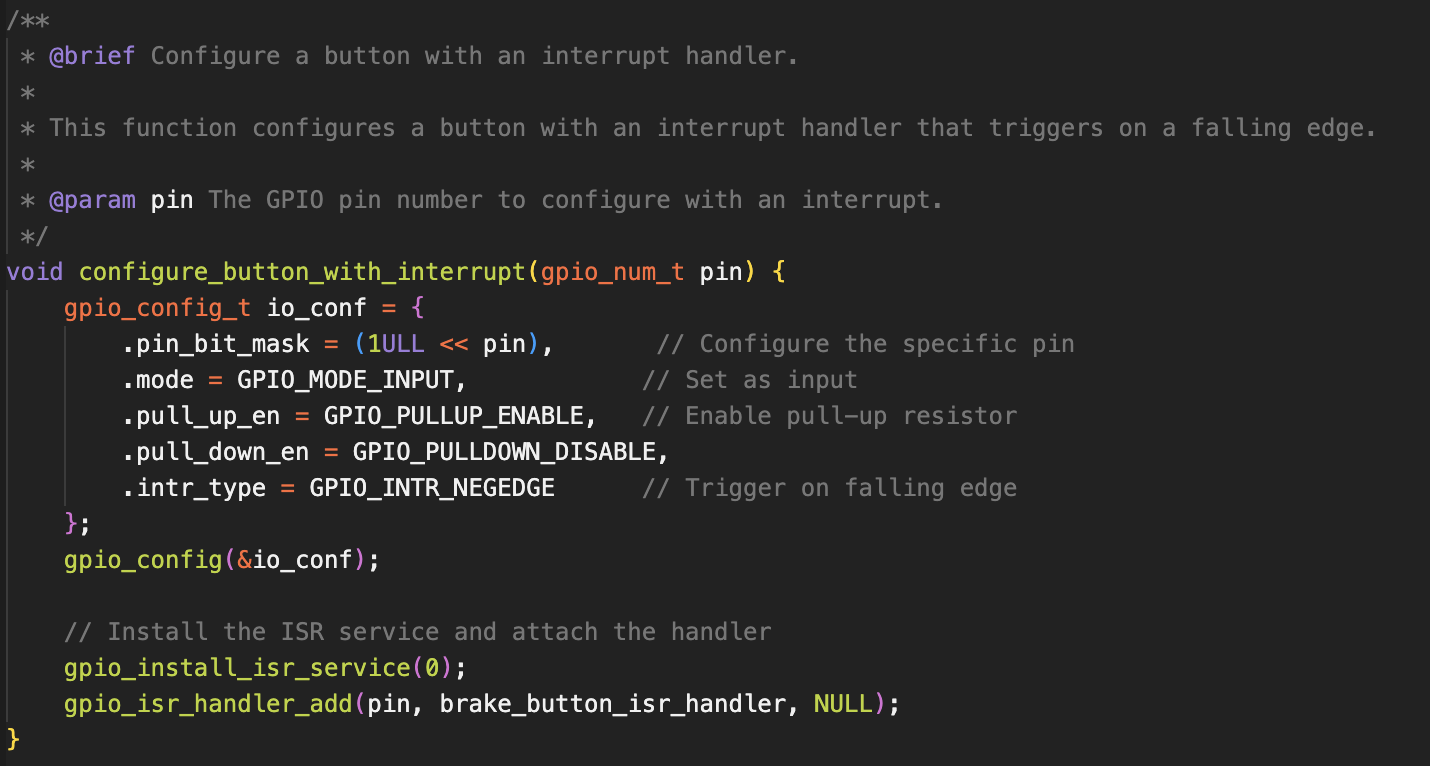
\includegraphics[scale=0.25]{img/configure.png}

\subsubsection{Using a DC Motor for the First Time}
Using a DC motor with the L293D motor driver for the first time was also an exciting part of the project. I had never worked with a motor controller before, and getting the motor to work with a controller like that was really cool. It was really fun to do quite a bit of research on how to simply connect stuff.

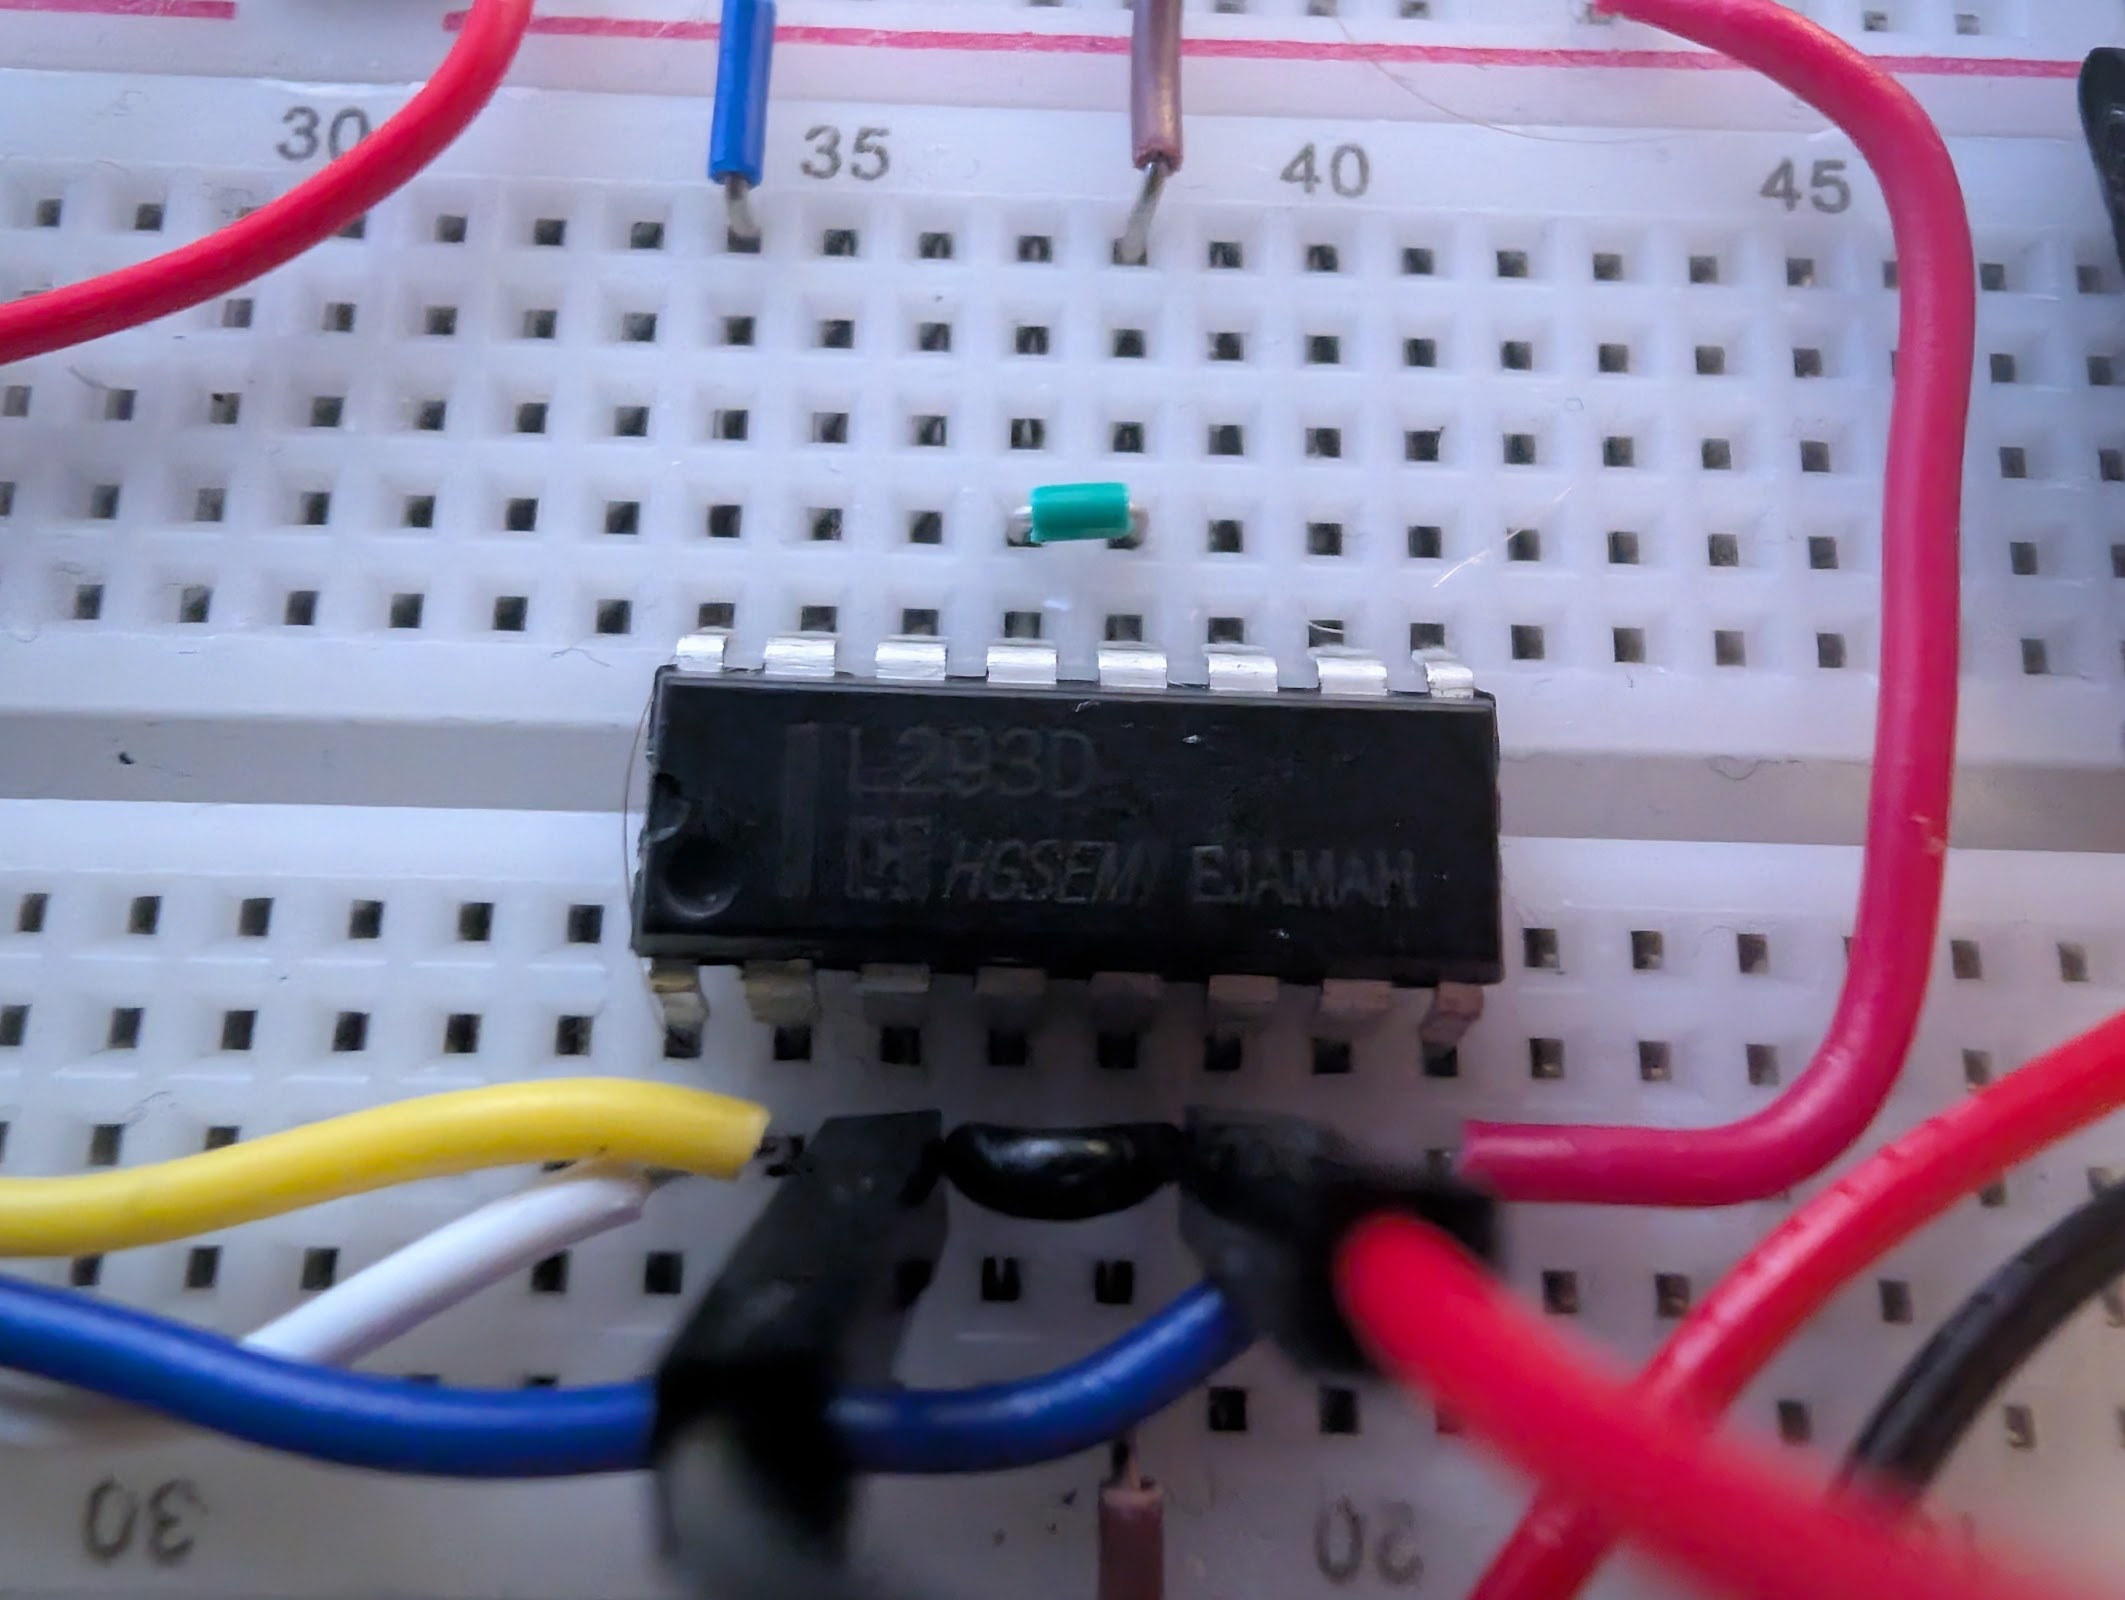
\includegraphics[scale=0.10]{img/L293D.png}

\subsubsection{Overall Project Experience}
Overall, this project was a significant step in my embedded systems journey. It allowed me to dive into areas I had not explored before, and despite the challenges, it was really cool to see most things come together. I just wish I could've made the OLED screen work how I wanted it to.

\newpage
